% !TEX TS-program = latexmk 

\documentclass[12pt,twoside,spanish]{book}

% Verificacion de sintaxis sin producir salida:
% descomentar la segunda linea para verificar
% sintaxis sin producir salida.
\usepackage{syntonly}
% \syntaxonly

% Palabras clave en distintos idiomas
\usepackage[activeacute]{babel}

% Patrones para division en silabas
\hyphenation{par-ti-cu-lar}

% Inclusion de imagenes
\usepackage{graphicx}

% Codificacion de simbolos
\usepackage[T1]{fontenc}
\usepackage[applemac]{inputenc}

% Fuentes y simbolos adicionales
\usepackage{amsfonts}
\usepackage{amsmath}
\usepackage{amssymb}
\usepackage{mathrsfs}

% Colores
\usepackage[table]{xcolor}

\definecolor{verdeOscuro}{rgb}{0,0.6,0}
\definecolor{verdeAzulado}{RGB}{3,168,108}
\definecolor{gris}{rgb}{0.5,0.5,0.5}
\definecolor{malva}{rgb}{0.58,0,0.82}
\definecolor{grisClaro}{rgb}{0.92,0.92,0.92}

% Vinculos
\usepackage{hyperref}
\hypersetup{
  colorlinks,
  urlcolor={malva}
}

% Codigo
\usepackage{listings}
\lstset{
  language=[LaTeX]TeX,
  aboveskip=3mm,
  belowskip=3mm,
  showstringspaces=false,
  columns=flexible,
  basicstyle={\small\ttfamily},
  numbers=none,
  extendedchars=true,
  numberstyle=\tiny\color{gris},
  keywordstyle=\color{blue},
  commentstyle=\color{verdeOscuro},
  stringstyle=\color{malva},
  breaklines=true,
  breakatwhitespace=true,
  tabsize=3,
  backgroundcolor=\color{grisClaro},
  moretexcs={color},
}


% Algoritmos
\usepackage[ruled,lined,linesnumbered,commentsnumbered]{algorithm2e}

%\usepackage[all]{xy}

% Generacion de dibujos con TeX
\usepackage{tikz}
\usetikzlibrary{arrows,shapes,matrix,decorations,calc,positioning}
\tikzstyle{arc}   =[->,shorten <=3pt, shorten >=3pt,
                   >=stealth, line width=1.1pt]
\tikzstyle{edge}  =[shorten <=2pt, shorten >=2pt,
                    >=stealth, line width=1.1pt]
\tikzstyle{myloop}=[style={},shorten <=1pt, shorten >=1pt,
                    >=stealth, line width=1.1pt, loop]
\tikzstyle{vertex}=[circle, draw, minimum size=6pt,
                    line width=0.75pt, inner sep=0pt,
                    outer sep=0pt]


% Ajuste de parametros en la pagina
\usepackage{geometry}

% Ubicacion precisa de floats
\usepackage{float}

% Manejo de encabezados
\usepackage{fancyhdr}

% Estilo de encabezados
\pagestyle{fancy}
\renewcommand{\chaptermark}[1]{\markboth{#1}{}}
\renewcommand{\sectionmark}[1]{\markright{\thesection\ #1}}
\fancyhf{}
\fancyhead[LE,RO]{\textsc{\bfseries\nouppercase\thepage}}
\fancyhead[LO]{\textsc{\bfseries\nouppercase\rightmark}}
\fancyhead[RE]{\textsc{\bfseries\nouppercase\leftmark}}
\renewcommand{\headrulewidth}{0.5pt}
\renewcommand{\footrulewidth}{0pt}
\addtolength{\headheight}{3pt}
\fancypagestyle{plain}{
  \fancyhead{}
  \renewcommand{\headrulewidth}{0pt}
}

% Delimitadores para terminar las demostraciones
\newcommand{\blackqed}{\hfill$\blacksquare$}
\newcommand{\whiteqed}{\hfill$\square$}
\newcounter{proofcount}

% Generacion de tabla de contenidos
\usepackage{makeidx}
\makeindex

% Ambientes de teorema y demostracion
\usepackage{amsthm}

% Referencias con nombres automaticos
\usepackage{cleveref}

% Definiciones de nuevos ambientes
\newtheorem{teorema}{Teorema}[section]
\newtheorem{lema}[teorema]{Lema}
\newtheorem{proposicion}[teorema]{Proposici\'on}
\newtheorem{corolario}[teorema]{Corolario}

\theoremstyle{definition}
\newtheorem{definicion}[teorema]{Definici\'on}

% Nombres para cleveref
\crefname{teorema}{el Teorema}{los Teoremas}
\crefname{lema}{el Lema}{los Lemas}
\crefname{proposicion}{la Proposici\'on}{las Proposiciones}
\crefname{corolario}{el Corolario}{los Corolarios}
\crefname{algorithm}{el Algoritmo}{los Algoritmos}
\crefname{section}{la Secci\'on}{las Secciones}
\crefname{figure}{la Figura}{las Figuras}

% Redefinicion para que las demostraciones terminen con cuadrito negro
\renewenvironment{proof}[1][\proofname.]{\par
\ifnum \theproofcount>0 \pushQED{\whiteqed} \else \pushQED{\blackqed} \fi%
\refstepcounter{proofcount}
%
\normalfont %\topsep6\p@\@plus6\p@\relax
\trivlist
\item[\hskip\labelsep
\itshape
\textbf{\textit{#1}}]\ignorespaces
}{%
\addtocounter{proofcount}{-1}
\popQED\endtrivlist
}

% Macros
% Abreviatura para fuentes true type
\newcommand{\ttt}[1]{%
\texttt{#1}%
}

\newcommand{\indice}[1]{%
\textbf{#1}\index{#1}%
}

\newcommand{\indiceSub}[2]{%
\textbf{#2}\index{#1!#2}%
}

\begin{document}

\frontmatter

%%
%% Portada creada por la Facultad de Ciencias
%%

%%
%% Esqueleto para la portada de las tesis para
%% la Facultad de Ciencias de la UNAM
%%


%%%%%%%%%%%%%%%%%%%%%%%%%%%%%%%%%%%%%%%%%%%%%%%%%%%%%%%
%% Comandos para la portada

\newcommand{\titulo}[1]{\def\eltitulo{#1}}
%* la carrera corresponde al tí­tulo otorgado -Matemático-
%* NO AL NOMBRE DE LA CARRERA -Matemáticas- --RRP
\newcommand{\carrera}[1]{\def\lacarrera{#1}}
\newcommand{\nombre}[1]{\def\elnombre{#1}}      %* Del alumno
\newcommand{\director}[1]{\def\eldirector{#1}}  %* De tesis
\newcommand{\fecha}[1]{\def\lafecha{#1}}

%% Llene los siguientes datos (use MAYÚSCULAS)
%% Estos datos aparecerán en la portada y los encabezados
\titulo{T\'ITULO DE LA TESIS}
\nombre{\uppercase{NOMBRE COMPLETO}}
\carrera{T\'ITULO OTORGADO}
\director{\uppercase{C\'ESAR HERN\'ANDEZ CRUZ}}
\fecha{2021}


\thispagestyle{empty}

%% Barra izquierda - Escudos
\hskip-1.5cm
\begin{minipage}[c][10cm][s]{3cm}
  \begin{center}
    
\includegraphics[height=2.6cm]{escudo-unam}\\[10pt]
    \hskip2pt\vrule width2pt height13cm\hskip1mm
    \vrule width1pt height13cm\\[10pt]
    
\includegraphics[height=2.6cm]{escudo-ciencias}
  \end{center}
\end{minipage}\quad
%% Barra derecha - Tí­tulos
\begin{minipage}[c][9.5cm][s]{10cm}
  \begin{center}
    % Barra superior
    {\large \scshape Universidad Nacional Aut\'onoma de M\'exico}
    \vspace{.3cm}
    \hrule height2pt
    \vspace{.1cm}
    \hrule height1pt
    \vspace{.3cm}
    {\scshape Facultad de Ciencias}

    % Titulo del trabajo
    \vspace{3cm}

    {\Large \eltitulo}

    \vspace{3cm}

    % Tipo de trabajo
    \makebox[8cm][s]{\Huge T E S I S}\\[8pt]
    QUE PARA OBTENER EL T\'ITULO DE:\\[3pt]
    \mbox{}\lacarrera\\[13pt]
    PRESENTA:\\[3pt]
    \elnombre

    \vspace{2cm}

    {\small DIRECTOR DE TESIS:\\ \eldirector}

    \vspace{2cm}

    \lafecha

  \end{center}
\end{minipage}

{\small
\begin{quote}
\begin{tabular}{lll}
1.Datos del alumno          & {}                                          \\
Apellido paterno            & Paterno                                     \\
Apellido materno            & Materno                                     \\
Nombre(s)                   & Nombres                                     \\
Tel\'efono                  & XX XX XX XX XX                              \\
Universidad                 & Universidad Nacional Aut\'onoma de M\'exico \\
Facultad o escuela          & Facultad de Ciencias                        \\
Carrera                     & Carrera                                     \\
N\'umero de cuenta          & XXXXXXXXX                                   \\
{}                          & {}                                          \\
2. Datos del tutor          & {}                                          \\
Grado                       & Dr.                                         \\
Nombre(s)                   & C\'esar                                     \\
Apellido paterno            & Hern\'andez                                 \\
Apellido materno            & Cruz                                        \\
{}                          & {}                                          \\
3. Datos del sinodal 1      & {}                                          \\
Grado                       & Dra.                                        \\
Nombre(s)                   & Nombres                                     \\
Apellido paterno            & Paterno                                     \\
Apellido materno            & Materno                                     \\
{}                          & {}                                          \\
4. Datos del sinodal 2      & {}                                          \\
Grado                       & M. en C.                                    \\
Nombre(s)                   & Nombres                                     \\
Apellido paterno            & Paterno                                     \\
Apellido materno            & Materno                                     \\
{}                          & {}                                          \\
5. Datos del sinodal 3      & {}                                          \\
Grado                       & Mat.                                        \\
Nombre(s)                   & Nombres                                     \\
Apellido paterno            & Paterno                                     \\
Apellido materno            & Materno                                     \\
{}                          & {}                                          \\
6. Datos del sinodal 4      & {}                                          \\
Grado                       & Lic. en Ciencias de la Computaci\'on        \\
Nombre(s)                   & Nombres                                     \\
Apellido paterno            & Paterno                                     \\
Apellido materno            & Materno                                     \\
{}                          & {}                                          \\
7.Datos del trabajo escrito & {}                                          \\
T\'itulo                    & T\'itulo                                    \\
N\'umero de p\'aginas       & XX p.                                       \\
A\~no                       & 2021                                        \\
\end{tabular}
\end{quote}
}

\chapter*{Agradecimientos}
\addcontentsline{toc}{chapter}{Agradecimientos}

Agradezco a mi director de tesis por haber hecho esta plantilla.

\tableofcontents


\mainmatter

\chapter{Introducci\'on}
\label{sec:intro}

Este documento tiene algunos ejemplos m\'inimos de caracter\'isticas que se
suelen utilizar en tesis de las licenciaturas en matem\'aticas y ciencias de la
computaci\'on, en particular en el \'area de teor\'ia de gr\'aficas (el \'area
de trabajo del autor).

Se exhorta al usuario a leer la
\href{https://tobi.oetiker.ch/lshort/lshort.pdf}{Not So Short Inroduction to
\LaTeX}.   Aunque realmente no es un documento muy largo, para quienes nunca han
usado \LaTeX{} es posible que las partes t\'ecnicas no tengan sentido.   En este
caso, es recomendable leer los dos primeros cap\'itulos, y regresar al resto del
documento para hacer consultas, o cuando se tenga algo de experiencia y se
desee mejorar como usuario.   En particular, antes de intentar cambiar el tipo
de letra, o el tama\~no de los m\'argenes, considere la siguiente observaci\'on
que aparece en el documento antes mencionado:
\begin{quote}
  Typographical design  is  a  craft.   Unskilled  authors  often  commit
  seriousformatting errors  by  assuming  that  book  design  is  mostly  a
  question of aesthetics---``If a document looks good artistically, it is well
  designed.'' But as a document has to be read and not hung up in a picture
  gallery, the readability and understandability is of much greater importance
  than the beautiful look of it.
\end{quote}

Idealmente, el lector obtuvo esta plantilla mediante
\href{https://github.com/Japodrilo/template-tesis}{este repositorio}. De no ser
as\'i, se le invita a visitarlo, y a usar las bondades del control de versiones
que el uso de \href{https://git-scm.com/}{Git} otorga (en particular cuando se
utiliza en conjunto con alguna plataforma para albergar sus repositorios
remotamente\footnote{Los alumnos de la Facultad de Ciencias de la UNAM tienen
acceso al \href{https://education.github.com/pack}{GitHub Student Developer
Pack} con su cuenta \ttt{@ciencias.unam.mx}.}).


\section{C\'omo usar esta plantilla}
\label{sec:howto}

Esta plantilla se dise\~n\'o como una ayuda para aquellos usuarios que ya
est\'an familiarizados con \LaTeX, pero nunca han desarrollado un proyecto
``grande'' (m\'as all\'a de tareas o reportes finales de proyectos).   Siguiendo
las instrucciones encontradas en el archivo \ttt{README.md}, lo m\'as probable
es que hayan creado un nuevo repositorio a partir del ``template repository''
que contiene este proyecto.   En primer lugar, verifique que el proyecto compile
adecuadamente; el proyecto deber\'ia de compilar sin errores ni advertencias. Es
posible que la primera vez que se compila, su manejador de paquetes actualice
varios de \'estos, lo que puede llevar un tiempo.   En caso de tener errores, es
posible que \'estos se deban a la falta de algunos paquetes, y a que su
manejador de paquetes no los instala autom\'aticamente;  instalar los paquetes
faltantes manualmente deber\'ia de resolver todos los problemas.

La estructura de este proyecto es sencilla.   Hay un archivo central,
\ttt{tesis.tex}, que contiene el pre\'ambulo del documento, y donde se incluyen
todos los paquetes y definiciones necesarias.   El c\'odigo est\'a comentado,
explicando de forma m\'inima para qu\'e sirve cada comando; se recomienda que al
modificarlo se mantenga un estilo semejante para no causarle problemas
innecesarios a su yo del futuro.   Todos los contenidos se encuentran en otros
archivos dentro del mismo directorio, que son llamados desde \ttt{tesis.tex}
mediante el comando \ttt{\textbackslash{include}}.   De esta forma se
incluyen la car\'atula, la hoja de datos, los cap\'itulos que forman parte de la
tesis, la bibliograf\'ia, etc.   Por otro lado, \LaTeX~ genera (casi)
autom\'aticamente el \'indice y el \'indice alfab\'etico, pero hay que agregar
comandos para su inclusi\'on.  La mayor\'ia de los usuarios s\'olo necesitan
preocuparse por modificar algunos de los archivos existentes, e incluir otros.
Sin embargo, es \'util que est\'en familiarizados con los conceptos de
\ttt{frontmatter}, \ttt{mainmatter}, \ttt{appendix} y \ttt{backmatter} (puede
referirse a \cite{oetiker2007} para revisarlos).

A continuaci\'on, se recomienda revisar el documento generado (este documento) e
identificar cu\'ales son las caracter\'isticas que se desean utilizar (dibujos,
algoritmos, tablas, etc.).   Tras determinar cu\'ales son los paquetes
relevantes para las caracter\'isticas deseadas, comentar (o borrar) todos
aquellos que no ser\'an utilizados en el archivo \ttt{tesis.tex}.   Si se est\'a
usando \ttt{git}, se recomienda leer \cref{sec:git}.   De otro modo, puede
empezar a reemplazar los contenidos de la plantilla con su propio trabajo.

\section[Uso recomendado con git]{Flujo de trabajo recomendado con \ttt{git}}
\label{sec:git}

Si el lector no est\'a usando \ttt{git}\index{git}, puede ignorar esta
secci\'on.   De otro modo, se propone un flujo de trabajo con el que el tesista
puede autogestionar el desarrollo de su tesis, o \'este puede ser supervisado
por su director de tesis mediante el uso de \ttt{GitHub}\index{git!GitHub}.

Este repositorio cuenta con dos ramas al momento de ser clonado: \ttt{master} y
\ttt{original}.   Idealmente, \ttt{master} debe contener su trabajo final, una
vez que ha sido revisado por su director de tesis, por lo que nunca deber\'ia de
trabajar directamente sobre esta rama.   Por este motivo, antes de realizar
cambios y experimentos en los archivos del proyecto, se recomienda crear una
nueva rama, llamada por ejemplo \ttt{prueba}, usando el comando \ttt{git
checkout -b prueba}.   Tras realizar algunos experimentos, eliminar los
contenidos que no necesita, y agregar sus datos a la car\'atula y hoja de datos,
posiblemente se sienta listo para empezar a incluir su trabajo en el proyecto.
En este momento se recomienda agregar los cambios realizados al repositorio,
realizar un \ttt{commit} con los mismos, y realizar un \ttt{merge} a
\ttt{master}.   A partir de ahora, \ttt{master} estar\'a lista para empezar a
trabajar.

En este momento, es posible crear
\href{https://guides.github.com/features/issues/}{\ttt{Issues}} en su
repositorio para tener metas de trabajo.   Como muy posiblemente s\'olo una
persona est\'e trabajando en el proyecto (el tesista), es posible que s\'olo
se trabaje en un \ttt{issue} a la vez, sin embargo, es una buena pr\'actica
tener una rama para cada \ttt{issue} (lo que resultar\'a a\'un m\'as \'util si
se trabaja en m\'as de una caracter\'istica nueva a la vez).   Idealmente, toda
rama nueva saldr\'a de \ttt{master}, y estar\'a dedicada a resolver un \'unico
\ttt{issue}.   Un ciclo de trabajo\index{ciclo de trabajo} usual puede verse
de la siguiente forma.

\begin{enumerate}
  \item Determinar una caracter\'istica nueva que se desea agregar al
    trabajo (e.g., la demostraci\'on de un teorema central de la tesis).

  \item Crear un \ttt{issue} describiendo qu\'e es lo que espera agregar
    al trabajo (e.g., qu\'e conceptos se necesitan agregar, proveer una
    referencia del teorema, indicar si es necesario incluir resultados
    preliminares o ejemplos).

  \item Asignar el \ttt{issue} al tesista, y opcionalmente agregar una fecha
    l\'imite.   (En caso de que el director de tesis est\'e supervisando el
    trabajo mediante \ttt{git}, asignarlo como revisor del \ttt{issue}.)

  \item Crear una nueva rama (a partir de \ttt{master}) para resolver el
    \ttt{issue}.

  \item Una vez resuelto el \ttt{issue}, hacer un \ttt{commit} (o varios) con
    los cambios, un \ttt{push} al repositorio, y abrir un \ttt{pull request}
    que ser\'a cerrado una vez que el director de tesis haya revisado el nuevo
    trabajo. (En caso de que el director de tesis est\'e supervisando el
    trabajo mediante \ttt{git}, deber\'a de ser agregado como revisor del
    \ttt{pull request}, y \'este ser\'a mezclado hasta tener su aprobaci\'on.)

  \item Tras aceptar el \ttt{pull request}, cerrar el \ttt{issue} y borrar la
    rama correspondientes (esto puede hacerse autom\'aticamente al aceptar el
    \ttt{pull request}).
\end{enumerate}

Un ciclo de trabajo tomar\'a tipicamente una semana, por lo que las metas a ser
cubiertas por cada \ttt{issue} deber\'an planearse con cuidado.

Se recomienda no modificar la rama \ttt{original}.   Si en cualquier momento se
necesitara tener acceso a este documento (quiz\'a el usuario requiere revisar un
ejemplo, o recuperar alg\'un paquete que borr\'o previamente), basta con
cambiarse a la rama \ttt{original}, donde siempre habr\'a una copia local del
mismo.   Es importante se\~nalar que, por el momento, \ttt{GitHub} crea
historias distintas para todas las ramas en un repositorio plantilla, por lo que
no es posible mezclar f\'acilmente commits entre \ttt{original} y \ttt{master}.
Esperamos que en un futuro \ttt{GitHub} permita empezar todas las ramas en un
repositorio plantilla con el mismo commit, en cuyo caso se integrar\'a una
tercera rama (\ttt{prueba}) a este repositorio.

\chapter{Ejemplos}
\label{cap:ejemplos}

\section{Ambientes y etiquetas}
\label{sec:etiquetas}

Todos los ambientes que se desee referir por n\'umero m\'as adelante deben de
tener una etiqueta.  Consideremos por ejemplo el siguiente lema.

\begin{lema}
\label{lem:primero}
Primer lema de ejemplo.
\end{lema}

Seguido de un segundo lema.

\begin{lema}
\label{lem:segundo}
Segundo lema de ejemplo.
\end{lema}

Que se utilizan para demostrar \cref{teo:ejemplo}.

\begin{teorema}
\label{teo:ejemplo}
Primer teorema de ejemplo.
\end{teorema}

\begin{proof}
Se sigue de \cref{lem:primero,lem:segundo}.
\end{proof}

Y finalmente obtener el siguiente corolario.

\begin{corolario}
\label{cor:ejemplo}
Corolario de ejemplo.
\end{corolario}

Usando el paquete \href{http://tug.ctan.org/tex-archive/macros/latex/contrib/%
cleveref/cleveref.pdf}{\ttt{cleveref}}\index{cleveref} es posible referirse de
forma sencilla a \cref{lem:primero,lem:segundo,teo:ejemplo,cor:ejemplo} (ver el
c\'odigo correspondiente en \cref{fig:cref}, notando que se utiliz\'o el comando
\ttt{\textbackslash{cref}}).   Este paquete agrega de forma autom\'atica el
nombre del ambiente, e.g., ``el Teorema'', al n\'umero cuando se hace una
referencia.   Esto resulta bastante \'util cuando, por ejemplo, se decide que un
resultado que inicialmente se enunci\'o como un teorema, realmente deber\'ia de
ser un lema; no es necesario buscar todos los lugares donde la referencia
correspondiente ocurre y cambiar los nombres, pues \ttt{cleveref} se encarga de
hacer los cambios.

\begin{figure}[H]
  \centering
  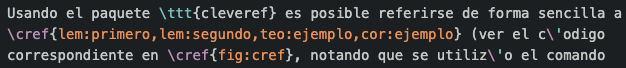
\includegraphics[width=0.8\textwidth]{recursos/capturas/cref}
  \caption{Ejemplo de uso de \ttt{\textbackslash{cref}}.}
  \label{fig:cref}
\end{figure}

Sin embargo, la gram\'atica del espa\~nol hace necesario introducir variantes en
algunos casos especiales, como cuando hacemos referencia ``al Teorema
\ref{teo:ejemplo}'' (n\'otese que se utiliz\'o ``al Teorema'' en lugar de ``el
Teorema''), o queremos decir que un resultado es una consecuencia ``del
Corolario \ref{cor:ejemplo}''.   En este caso, necesitamos agregar el nombre del
ambiente a mano, y usar el comando habitual \ttt{\textbackslash{ref}}.   El
autor del presente documento prefiere utilizar siempre may\'usculas cuando se
usa el nombre de un ambiente referido por n\'umero, e.g., ``\cref{teo:ejemplo}''
en lugar de ``el teorema \ref{teo:ejemplo}'', por lo que esta configuraci\'on se
ve reflejada en el archivo \ttt{tesis.tex}, cuando se utiliza el comando
\ttt{\textbackslash{crefname}} para definir los nombres de ambiente que debe de
usar \ttt{cleveref}.

Una alternativa para evitar algunos de los problemas descritos en el p\'arrafo
anterior es definir el nombre del ambiente sin utilizar el art\'iculo, e.g.,
``Teorema'' en lugar de ``el Teorema''.   Aunque esto permite un poco m\'as de
flexibilidad, cuando es necesario cambiar un ambiente con nombre masculino a uno
con nombre femenino, o viceversa (por ejemplo proposici\'on por lema), es
necesario realizar todos los cambios de los art\'iculos a mano.  Adicionalmente,
(y el motivo principal por el que se decidi\'o no usar esta variante) el uso del
paquete como el mostrado en el ejemplo de \cref{fig:cref} dejar\'ia de
funcionar, pues los art\'iculos ser\'ian omitidos, generando una construcci\'on
gramatical incorrecta.

Si no se desea usar el paquete \ttt{cleveref}, siempre puede omitirse y utilizar
\'unicamente el comando \ttt{\textbackslash{ref}} que est\'a incluido por
omisi\'on en \LaTeX.

Adem\'as de los ambientes, tambi\'en es posible etiquetar cap\'itulos o
secciones, y referirnos a la p\'agina donde aparece una etiqueta dada.   Por
ejemplo, podemos referirnos a \cref{sec:dibujos} en la \cpageref{sec:dibujos}, o
al Cap\'itulo \ref{cap:ejemplos}.   La referencia a las p\'aginas es \'util en
la versi\'on impresa del documento, aunque en la versi\'on digital parezca un
poco in\'util gracias a que cada referencia es una liga al objeto en cuesti\'on.



\section{Dibujos y colores}
\label{sec:dibujos}

Los dibujos pueden agregarse de al menos dos formas obvias.   La primera es
hacerlos dentro de \LaTeX con alg\'un paquete como
\href{https://github.com/pgf-tikz/pgf}{\ttt{tikz}}\index{tikz}.   La segunda es
generarlos con alg\'un recurso externo, e incluirlo con el comando
\ttt{\textbackslash{includegraphics}}.   Tambi\'en puede usarse una
combinaci\'on de ambos, generando un PDF con la imagen en un archivo externo de
\LaTeX, y agreg\'andolo con \ttt{\textbackslash{includegraphics}}; una ventaja
de esta tercera posibilidad es que el compilador realiza menos trabajo para
generar el documento.

En \cref{fig:grafica} podemos ver un ejemplo de un dibujo hecho con \ttt{tikz}.
Una ventaja de hacer los dibujos dentro de \LaTeX{} es que resulta f\'acil
agregar f\'ormulas o etiquetas con la misma tipograf\'ia que el resto del
documento.

\begin{figure}[ht!]
\centering
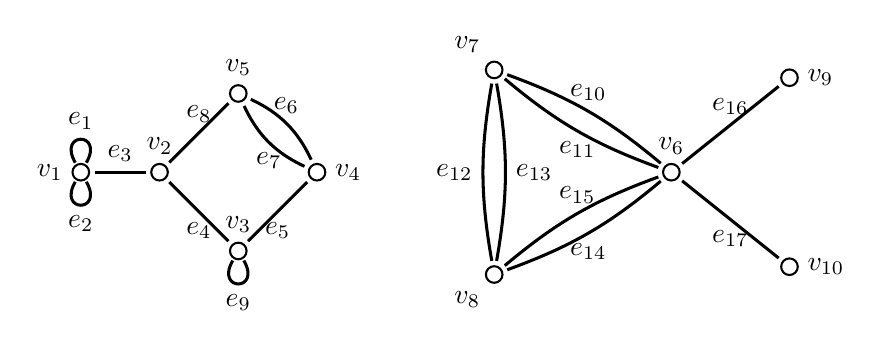
\begin{tikzpicture}
\node (0) [vertex,label=180:$v_1$] at (0,0){};
\node (1) [vertex,label=90:$v_2$]  at (1,0){};
\begin{scope}[xshift=2cm]
\node (2) [vertex,label=90:$v_3$]  at (270:1){};
\node (3) [vertex,label=0:$v_4$]   at (0:1){};
\node (4) [vertex,label=90:$v_5$]  at (90:1){};
\end{scope}

\draw [myloop,in=60,out=120,looseness=12]
      (0) to node[above]{$e_1$} (0);
\draw [myloop,in=240,out=300,looseness=12]
      (0) to node[below]{$e_2$} (0);
\draw [myloop,in=240,out=300,looseness=12]
      (2) to node[below]{$e_9$} (2);

\draw [edge]               (0) to node [above] {$e_3$} (1);
\draw [edge]               (1) to node [below] {$e_4$} (2);
\draw [edge]               (2) to node [below] {$e_5$} (3);
\draw [edge,bend right=20] (3) to node [above] {$e_6$} (4);
\draw [edge,bend left=20]  (3) to node [below] {$e_7$} (4);
\draw [edge]               (4) to node [above] {$e_8$} (1);


% Componente derecha
\begin{scope}[xshift=6cm]
\node (5) [vertex,label=90:$v_6$]    at (0:1.5){};
\node (6) [vertex,label=120:$v_7$]   at (120:1.5){};
\node (7) [vertex,label=240:$v_8$]   at (240:1.5){};
\node (8) [vertex,label=0:$v_9$]     at (3,1.2){};
\node (9) [vertex,label=0:$v_{10}$]  at (3,-1.2){};

\draw [edge,bend right=10] (5) to node [above] {$e_{10}$} (6);
\draw [edge,bend left=10]  (5) to node [below] {$e_{11}$} (6);
\draw [edge,bend right=10] (6) to node [left]  {$e_{12}$} (7);
\draw [edge,bend left=10]  (6) to node [right] {$e_{13}$} (7);
\draw [edge,bend right=10] (7) to node [below] {$e_{14}$} (5);
\draw [edge,bend left=10]  (7) to node [above] {$e_{15}$} (5);
\draw [edge]               (5) to node [above] {$e_{16}$} (8);
\draw [edge]               (5) to node [below] {$e_{17}$} (9);
\end{scope}

\end{tikzpicture}
\caption{El diagrama de una gr\'afica con lazos y
aristas m\'ultiples.}
\label{fig:grafica}
\end{figure}

Es f\'acil agregar colores a los dibujos.   Hay que tener presente que
\ttt{tikz} construye el dibujo por capas, y el c\'odigo se ejecuta de forma
secuencial, por lo que la \'ultima parte del c\'odigo es la \'ultima capa que se
dibujar\'a, y puede cubrir a otras, generando un resultado distinto al deseado.
Es posible definir colores nuevos mediante el comando
\ttt{\textbackslash{definecolor}}, en el caso de este documento, todos los
colores nuevos se definen en el archivo \ttt{tesis.tex}.   Las diferentes
opciones para el comando \ttt{\textbackslash{definecolor}} se encuentran
explicadas \href{https://en.wikibooks.org/wiki/LaTeX/Colors}{aqu\'i}.

Para agregar colores en el texto, o en las celdas de una tabla, u otros lugares,
se puede utilizar el paquete
\href{https://ctan.org/pkg/xcolor}{\ttt{xcolor}}\index{xcolor}.  Una forma
sencilla de usar color en el texto es con la construcci\'on
\begin{lstlisting}
{\color{nombre-del-color}texto con color}}
\end{lstlisting}
{\color{verdeAzulado}lo que permite generar texto de color.

Incluso es posible usar un color a lo largo de distintos p\'arrafos.}


\begin{figure}[ht!]
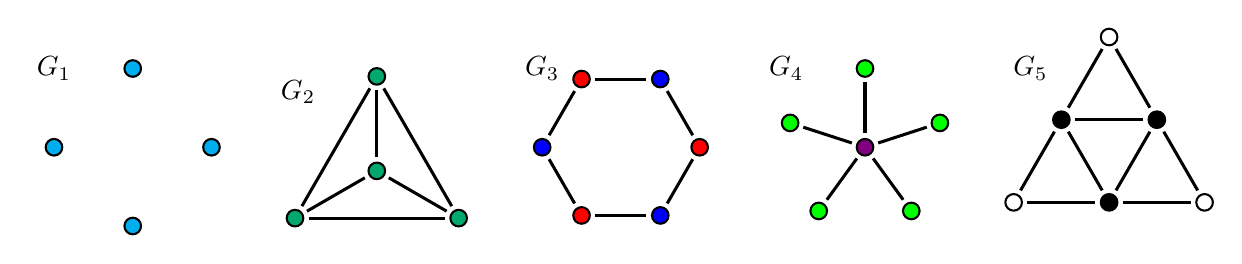
\begin{tikzpicture}
%%%%%%%%%%%%%%%%%%%%%%%%%%%%%%%%%%%%%%%%%%%%%%%%
%%%%%%%%%%         Empty Graph        %%%%%%%%%%
%%%%%%%%%%%%%%%%%%%%%%%%%%%%%%%%%%%%%%%%%%%%%%%%
\begin{scope}
% if label is needed -> label={(360/4)*\i}:$\i$
\foreach \i in {0,...,3}
	\node (\i) [vertex,fill=cyan] at ({(360/4)*\i}:1){};

\node (L) at (-1,1){$G_1$};
\end{scope}

%%%%%%%%%%%%%%%%%%%%%%%%%%%%%%%%%%%%%%%%%%%%%%%%
%%%%%%%%%%       Complete Graph       %%%%%%%%%%
%%%%%%%%%%%%%%%%%%%%%%%%%%%%%%%%%%%%%%%%%%%%%%%%
\begin{scope}[xshift=3.1cm,yshift=-0.3cm]
\node (4) [vertex,fill=verdeAzulado] at (0,0){};
\foreach \i in {0,1,2}
	\node (\i) [vertex,fill=verdeAzulado] at ({90+(360/3)*\i}:1.2){};

\foreach \i in {0,1,2}
	\draw [edge] let \n1={int(mod(\i+1,3))} in (\i) to (\n1);
\foreach \i in {0,1,2}
	\draw [edge] (\i) to (4);

\node (L) at (-1,1){$G_2$};
\end{scope}


%%%%%%%%%%%%%%%%%%%%%%%%%%%%%%%%%%%%%%%%%%%%%%%%
%%%%%%%%%%       Bipartite Graph      %%%%%%%%%%
%%%%%%%%%%%%%%%%%%%%%%%%%%%%%%%%%%%%%%%%%%%%%%%%
\begin{scope}[xshift=6.2cm,yshift=0cm]
\foreach \i in {0,2,4}
	\node (\i) [vertex,fill=red]  at ({(360/6)*\i}:1){};
\foreach \i in {1,3,5}
	\node (\i) [vertex,fill=blue] at ({(360/6)*\i}:1){};

\foreach \i in {0,...,5}
	\draw [edge] let \n1={int(mod(\i+1,6))} in (\i) to (\n1);

\node (L) at (-1,1){$G_3$};
\end{scope}


%%%%%%%%%%%%%%%%%%%%%%%%%%%%%%%%%%%%%%%%%%%%%%%%
%%%%%%%%%%            Star            %%%%%%%%%%
%%%%%%%%%%%%%%%%%%%%%%%%%%%%%%%%%%%%%%%%%%%%%%%%
\begin{scope}[xshift=9.3cm]
\node (6) [vertex,fill=violet] at (0,0){};
\foreach \i in {0,...,4}
	\node (\i) [vertex,fill=green] at ({90+(360/5)*\i}:1){};

\foreach \i in {0,...,4}
	\draw [edge] (\i) to (6);

\node (L) at (-1,1){$G_4$};
\end{scope}


%%%%%%%%%%%%%%%%%%%%%%%%%%%%%%%%%%%%%%%%%%%%%%%%
%%%%%%%%%%           Split            %%%%%%%%%%
%%%%%%%%%%%%%%%%%%%%%%%%%%%%%%%%%%%%%%%%%%%%%%%%
\begin{scope}[xshift=12.4cm]
\foreach \i in {0,2,4}
	\node (\i) [vertex,fill=black] at ({30+(360/6)*\i}:0.7){};
\foreach \i in {1,3,5}
	\node (\i) [vertex] at ({30+(360/6)*\i}:1.4){};

\foreach \i in {0,...,5}
	\draw [edge] let \n1={int(mod(\i+1,6))} in (\i) to (\n1);
\foreach \i in {0,2,4}
	\draw [edge] let \n1={int(mod(\i+2,6))} in (\i) to (\n1);

\node (L) at (-1,1){$G_5$};
\end{scope}

\end{tikzpicture}
\caption{Ejemplos de gr\'aficas vac\'ia, completa,
bipartita, bipartita completa y escindible.}
\label{fig:fam1}
\end{figure}

Continuando con los dibujos, resulta bastante \'util usar ciclos \ttt{for}
dentro de \ttt{tikz} para realizar dibujos que tienen simetr\'ias.   Un ejemplo
de esto ocurre en \cref{fig:fam1}.   En \cref{fig:tikzFor}, se observa el
c\'odigo del ciclo azul y rojo que aparece en \cref{fig:fam1}.

\begin{figure}[ht!]
  \centering
  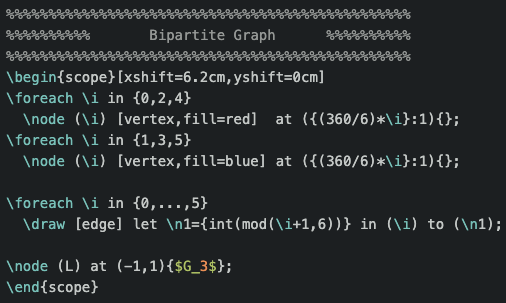
\includegraphics[width=0.8\textwidth]{recursos/capturas/tikzfor}
  \caption{Ejemplo de un ciclo \ttt{for} dentro de \ttt{tikz}.}
  \label{fig:tikzFor}
\end{figure}

Aunque en este caso los ejemplos se concentran en dibujar gr\'aficas, las
posibilidades de \ttt{tikz} son gigantescas.   Se recomienda al usuario revisar
el \href{https://mirror.las.iastate.edu/tex-archive/graphics/pgf/base/doc/%
pgfmanual.pdf}{manual de PGF y TikZ}.


\section{Algoritmos}

Para los algoritmos utilizamos el paquete \href{https://www.ctan.org/pkg/%
algorithm2e}{\ttt{algorithm2e}}\index{algorithm2e}.   En este caso simplemente
se presentar\'a un ejemplo de uso con un subconjunto limitado de las distintas
opciones que se pueden utilizar.   Se recomienda revisar la documentaci\'on del
paquete para conocer todas las posibilidades.

\begin{algorithm}[ht!]
\SetAlgorithmName{Algoritmo}{}
  \DontPrintSemicolon
  \SetKwData{False}{false}\SetKwData{True}{true}
  \SetKwFunction{New}{new}\SetKwFunction{End}{end}\SetKwFunction{Used}{used}
  \SetKwInOut{Input}{input}\SetKwInOut{Output}{output}

  \KwIn{Una gr\'afica conexa $G$ con un v\'ertice distingido $r$.}
  \KwOut{Funciones de parentesco $p$, nivel $\ell$ y tiempo de exploraci\'on
         $t$.}
  \BlankLine
  $Q \leftarrow []$; $i \leftarrow 0$\;
  $i \leftarrow i+1$\;
  colorear a $r$ de negro\;
  a\~nadir $r$ al final de $Q$\;
  $t(r) \leftarrow i$, $p(r) \leftarrow \varnothing$, $\ell (r) \leftarrow 0$\;
  {\While{$Q \ne []$}{
  	elegir a la cabeza $x$ de $Q$\;
 	\If{$x$ tiene un vecino $y$ sin colorear}{
		$i \leftarrow i+1$\;
		colorear a $y$ de negro\;
		a\~nadir $y$ al final de $Q$\;
		$t(y) \leftarrow i$, $p(y) \leftarrow x$, $\ell(y) \leftarrow \ell(x) + 1$\;
	}\Else{
		eliminar $x$ de $Q$\;
	}
  }
  }
  {\Return $(p,\ell,t)$}
  \caption{Breadth First Search}
  \label{alg:bfs}
\DecMargin{1em}
\end{algorithm}

\Cref{alg:bfs} muestra algunas opciones sencillas del paquete.   Quiz\'a la
observaci\'on m\'as importante para considerar respecto a \ttt{algorithm2e} es
que, por dise\~no, el paquete no divide los algoritmos para aparecer en m\'as
de una p\'agina.   Por lo tanto, un algoritmo largo usualmente se recorrer\'a
a la siguiente p\'agina (y posiblemente ocupar\'a una p\'agina completa).

\section{\'Indice alfab\'etico}
\label{sec:indice}

Es posible agregar palabras al \'indice\index{indice@\'indice} alfab\'etico
usando el comando \ttt{\textbackslash{index}}.   Un uso t\'ipico es el
siguiente; supongamos que se desea agregar la palabra ``gr\'afica'' al \'indice,
entonces es necesario escribir la palabra, seguida de la misma palabra dentro
del comando.
\begin{lstlisting}
gr\'afica\index{gr\'afica}
\end{lstlisting}

Cuando se introduce un concepto nuevo, es deseable resaltarlo de alguna forma en
el texto.   En los art\'iculos usualmente se utilizan \textit{cursivas} y en los
libros (o una tesis), generalmente se prefieren las \textbf{negritas}.   Por
este motivo, se agreg\'o al pre\'ambulo un comando para poner, al mismo tiempo,
una palabra en negritas y agregarla al \'indice; el comando es
\ttt{\textbackslash{indice}}.   Por ejemplo, dicho comando est\'a siendo
utilizado en la palabra \indice{concepto}, mismo que se puede verificar aparece
en el \'indice anal\'itico al final del documento. Tambi\'en es com\'un
encontrar una versi\'on especializada de un concepto, e.g., la definici\'on de
gr\'afica bipartita depende de la de gr\'afica.   En este sentido, es deseable
que ``gr\'afica bipartita'' aparezca como una entrada que depende de
``gr\'afica''.   Para lograr esto se utiliza el mismo comando
\ttt{\textbackslash{index}}, con la siguiente sintaxis.
\begin{lstlisting}
\index{concepto!subconcepto}
\end{lstlisting}

De manera an\'aloga al caso del comando \ttt{\textbackslash{indice}}, se cre\'o
un comando \ttt{\textbackslash{indiceSub}}, que toma dos argumentos.  El primero
es la entrada principal que aparecer\'a en el \'indice (e.g., gr\'afica), y la
segunda es la versi\'on especializada que depende de la primera (e.g.,
bipartita).   Para brindar libertad en la forma de redactar las definiciones,
\ttt{\textbackslash{indiceSub}} s\'olo imprime en el documento el segundo
argumento.   Por ejemplo, en \indiceSub{concepto}{subconcepto} se utiliz\'o
\ttt{\textbackslash{indiceSub}} con los argumentos \ttt{concepto} y
\ttt{subconcepto} (puede verificarse el funcionamiento en el \'indice).

Dependiendo del editor que se est\'e utilizando para trabajar con \LaTeX, es
posible que el \'indice no se actualice autom\'aticamente.   De ser el caso,
basta con ejecutar el siguiente comando en el directorio del proyecto donde se
encuentre el archivo \ttt{tesis.idx} (\'este \'ultimo se genera
autom\'aticamente al compilar \ttt{tesis.tex}).
\lstset{language=bash}
\begin{lstlisting}
makeindex tesis.idx
\end{lstlisting}

El comando anterior generar\'a el archivo \ttt{tesis.ind}, mismo que contiene la
informaci\'on necesaria para incluir el \'indice en el PDF final.

Los conceptos aparecen en orden alfab\'etico en el \'indice, sin embargo, el uso
de caracteres especiales (como letras acentuadas) afecta el orden habitual.
Para corregir problemas derivados del uso de caracteres especiales, se refiere
al lector al siguiente \href{https://en.wikibooks.org/wiki/LaTeX/%
Indexing#Using_special_characters}{art\'iculo sobre indexaci\'on}.



\backmatter

\printindex
\begin{thebibliography}{99}
\addcontentsline{toc}{chapter}{Bibliograf\'ia}

\bibitem{bondy2008}
  J.~A.~Bondy y U.~S.~R.~Murty,
  \textbf{Graph Theory},
  Springer, 2008.

\bibitem{corneilDAM3}
  D.~Corneil, H.~Lerchs y L.~Stewart~Burlingham,
  \textit{Complement reducible graphs},
  Discrete Applied Mathematics 3 (1981) 163--174.

\bibitem{diestel2017}
  R.~Diestel,
  \textbf{Graph Theory, Fifth Edition},
  Springer, 2017.

\bibitem{jonesTCS713}
  A.~Jones, F.~Protti y R.~R.~Del-Vecchio,
  \textit{Cograph generation with linear delay},
  Theoretical Computer Science 713 (2018) 1--10.

\bibitem{oetiker2007}
  T.~Oetiker, H.~Partl, I.~Hyna, and E.~Schlegl,
  The Not So Short Introduction to \LaTeX{} Version 6.4 (2021),
  \href{https://tobi.oetiker.ch/lshort/lshort.pdf}{%
  https://tobi.oetiker.ch/lshort/lshort.pdf}.

\end{thebibliography}


\end{document}
